% ser-cite.tex

\documentclass[tikz, border=3pt]{standalone}

\usepackage[dvipsnames]{xcolor}
\usetikzlibrary{arrows.meta}
% Selected notation from predicates.tex / newcommands.tex.
\newcommand{\set}[1]{\{#1\}}
\newcommand{\tuple}[1]{\langle#1\rangle}
\newcommand{\Key}{{\sf K}}
\newcommand{\Val}{{\sf V}}
\newcommand{\Predicate}{{\sf P}}
\newcommand{\predread}{{\sf PR}}
\newcommand{\itemwrite}{{\sf W}}
\newcommand{\match}{\Delta}
\newcommand{\T}{\mathcal{T}}
\newcommand{\History}{\mathcal{H}}
\newcommand{\G}{\mathcal{G}}
\newcommand{\VIS}{\mathsf{VIS}}
\newcommand{\AR}{\mathsf{AR}}
\newcommand{\SO}{\mathsf{SO}}
\newcommand{\WR}{\mathsf{WR}}
\newcommand{\WW}{\mathsf{WW}}
\newcommand{\RW}{\mathsf{RW}}
\newcommand{\PredWR}{\mathsf{PredWR}}
\newcommand{\PredRW}{\mathsf{PredRW}}
\newcommand{\PredRWCAV}{\mathsf{PredRW}^{+}}
\newcommand{\PredRWarXiv}{\mathsf{PredRW}^{-}}
\newcommand{\si}{\mathsf{SI}}
\newcommand{\ser}{\mathsf{SER}}
\newcommand{\rel}[1]{\xrightarrow{#1}}
\newcommand{\ncite}[1]{\textcolor{black!55}{\scriptsize\cite{#1}}}


% Standalone figures do not run the presentation bibliography pipeline.  These
% local labels let \ncite render the corresponding author--year citations.
\makeatletter
\newcommand{\declarecite}[2]{\expandafter\gdef\csname b@#1\endcsname{#2}}
\makeatother
\declarecite{CC:Bernstein1987}{Bernstein et al., 1987}
\declarecite{TP:Gray1993}{Gray and Reuter, 1993}
\declarecite{Adya:PhDThesis1999}{Adya, 1999}
\declarecite{Adya:ICDE2000}{Adya et al., 2000}
\declarecite{MakingSISER:TODS2005}{Fekete et al., 2005}
\declarecite{Emme:EuroSys2024}{Emmi et al., 2024}
\declarecite{Vbox:arXiv2025}{Zhou et al., 2025}
\declarecite{Emme:TOCS2026}{Emmi et al., 2026}

\begin{document}
  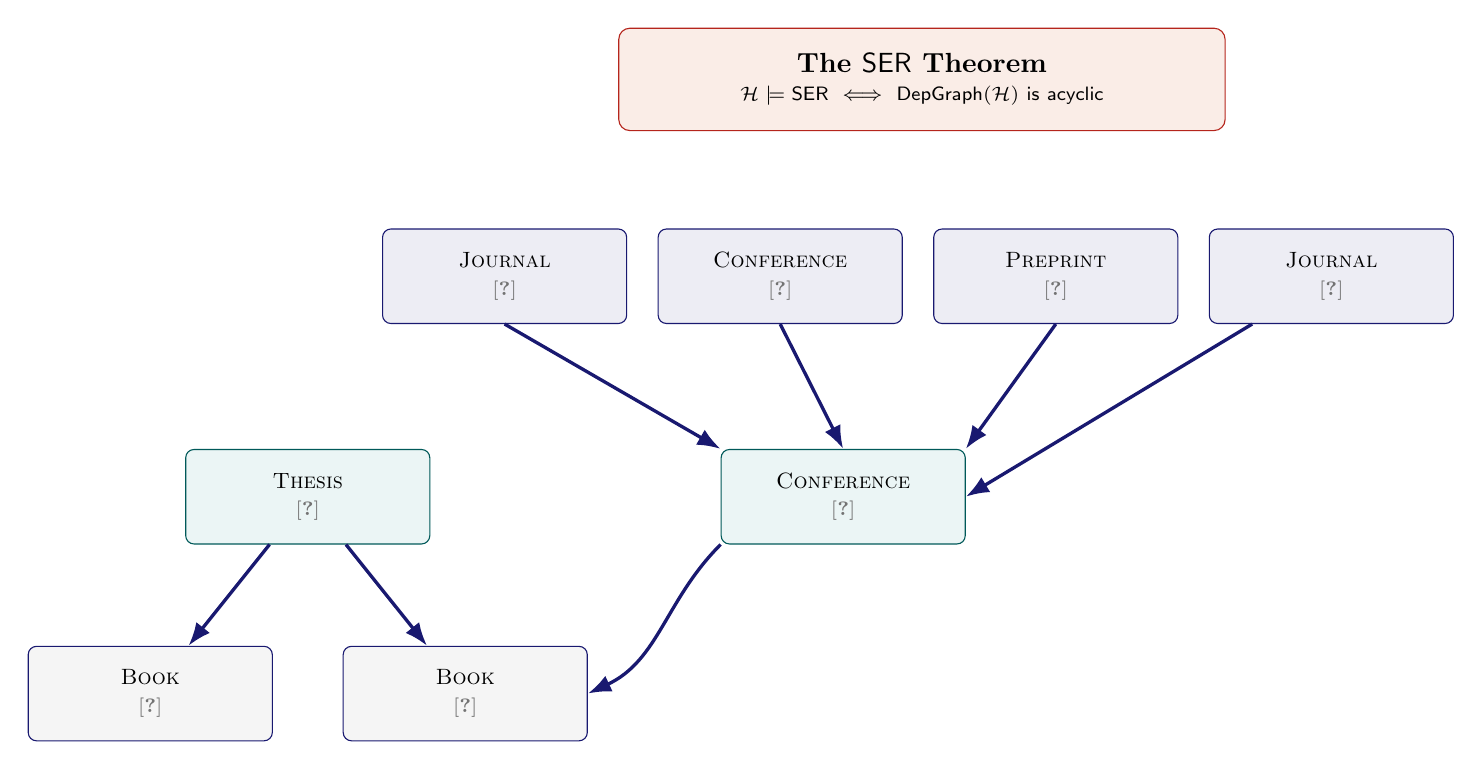
\begin{tikzpicture}[
      cite edge/.style={-Latex, very thick, MidnightBlue},
      citation/.style={
        draw = MidnightBlue,
        rounded corners = 3pt,
        fill = MidnightBlue!5,
        minimum width = 31mm,
        minimum height = 12mm,
        align = center,
        inner sep = 2mm,
      },
      foundation/.style={citation, fill = black!4},
      bridge/.style={citation, draw = teal!70!black, fill = teal!8},
      recent/.style={citation, fill = MidnightBlue!8},
      theorem/.style={
        draw = BrickRed,
        rounded corners = 4pt,
        fill = BrickRed!6,
        minimum width = 77mm,
        minimum height = 13mm,
        align = center,
      },
    ]
    \node[foundation] (gray) at (0, 0)
      {\footnotesize\textsc{Book}\\[-.2em]\ncite{TP:Gray1993}};
    \node[foundation] (cc) at (40mm, 0)
      {\footnotesize\textsc{Book}\\[-.2em]\ncite{CC:Bernstein1987}};

    \node[bridge] (thesis) at (20mm, 25mm)
      {\footnotesize\textsc{Thesis}\\[-.2em]\ncite{Adya:PhDThesis1999}};
    \node[bridge] (icde) at (88mm, 25mm)
      {\footnotesize\textsc{Conference}\\[-.2em]\ncite{Adya:ICDE2000}};

    \node[recent] (making) at (45mm, 53mm)
      {\footnotesize\textsc{Journal}\\[-.2em]\ncite{MakingSISER:TODS2005}};
    \node[recent] (emme) at (80mm, 53mm)
      {\footnotesize\textsc{Conference}\\[-.2em]\ncite{Emme:EuroSys2024}};
    \node[recent] (vbox) at (115mm, 53mm)
      {\footnotesize\textsc{Preprint}\\[-.2em]\ncite{Vbox:arXiv2025}};
    \node[recent] (order) at (150mm, 53mm)
      {\footnotesize\textsc{Journal}\\[-.2em]\ncite{Emme:TOCS2026}};

    \node[theorem] (ser) at (98mm, 78mm)
      {\textbf{The $\mathsf{SER}$ Theorem}\\[-.2em]
       \scriptsize $\mathcal{H}\models\mathsf{SER}\ \Longleftrightarrow\
       \mathsf{DepGraph}(\mathcal{H})\ \mathsf{is\ acyclic}$};

    % Each arrow points from the citing work to the cited work.
    \draw[cite edge] (thesis) -- (cc);
    \draw[cite edge] (thesis) -- (gray);
    \draw[cite edge] (icde.south west) to[out = 225, in = 25] (cc.east);
    \draw[cite edge] (making.south) -- (icde.north west);
    \draw[cite edge] (emme.south) -- (icde.north);
    \draw[cite edge] (vbox.south) -- (icde.north east);
    \draw[cite edge] (order) -- (icde.east);
  \end{tikzpicture}
\end{document}